\documentclass{article}
\usepackage[margin=1in]{geometry}
\usepackage{array}
\usepackage{graphicx}

\author{Carl Ehrett}
\title{Computer model calibration as a method of design}

\begin{document}

\maketitle

\section{Introduction}
% Discussion of computer experiments and computer model calibration. Lit review. Overview of project goals.

\subsection{Computer experiments}

\subsection{Computer model calibration}

\subsubsection{Gaussian processes}

\paragraph{Background}



\paragraph{Gaussian process regression}

\begin{figure}[h]
\centering
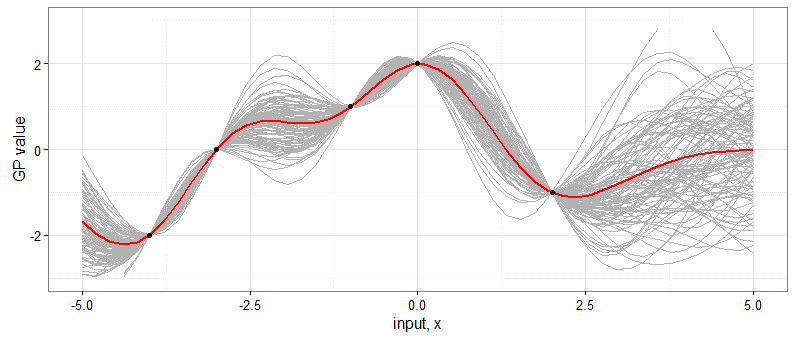
\includegraphics[width=.75\linewidth]{gp_example}
\caption{Example of a Gaussian process trained to interpolate five data points (black dots).}
\label{gp_example}
\end{figure}

\paragraph{Gaussian processes in computer model calibration}

\subsubsection{Markov chain Monte Carlo methods}

\paragraph{Background}

\paragraph{Metropolis-Hastings algorithm}

\paragraph{Elimination of boundary constraints}

\subsubsection{Normalization of inputs and standardization of outputs}
Blah

\subsubsection{Computational difficulties}
% And solutions
Blah

\paragraph{Likelihoods}
Blah

\paragraph{Ill-conditioned covariance matrices}

\section{Calibration for design}



\section{Application}

\subsection{Project background}

\subsection{Emulation of finite element simulator}
Blah

\subsubsection{Wind turbine blade simulator}
% Here the finite element model will be described
Blah

\subsubsection{Mathematical basis for the emulator}
% Includes formulae for trained mean and covariance functions
Blah

\subsubsection{Experimental design}
% How we selected the design points at which to observe the simulator
Blah

\subsubsection{Covariance parameters}
% How they were selected
Blah

\paragraph{Finding covariance parameters via MCMC}
% Why we didn't do it (computational difficulties
Blah

\paragraph{Grid optimization}
% Advantages and disadvantages; full grid and integration of lambda
Blah

\paragraph{Gradient method}
% Explanation and advantages
Blah

\begin{figure}
\centering
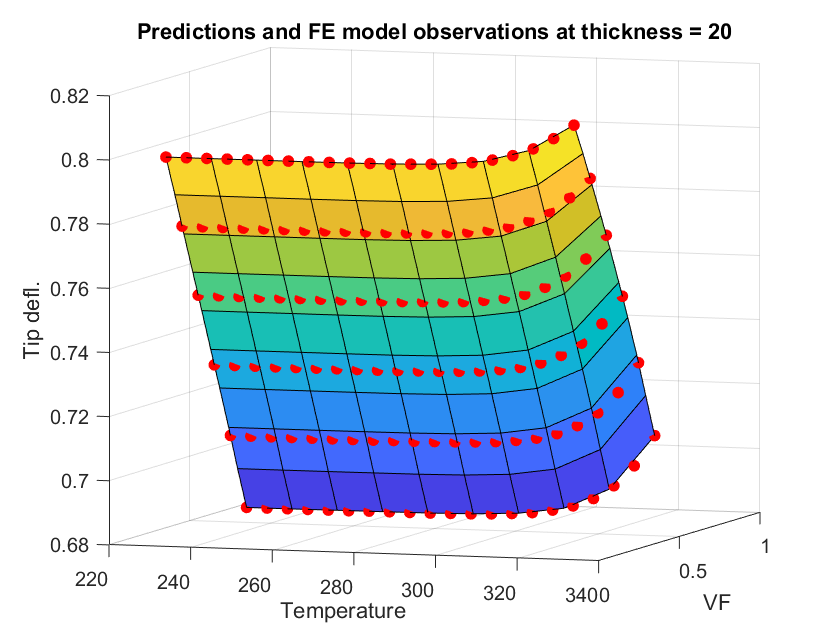
\includegraphics[width=.65\linewidth]{emulator_surface}
\caption{A slice of the GP emulator (restricted to the output for tip deflection) at thickness =20mm. Red dots are observations from the simulator.}
\label{fig:emulator_surface}
\end{figure}

\section{MCMC using the emulator}
Blah

\subsection{MCMC methods}
% Background on MCMC
Blah

\subsection{The model}
% Choice of priors and resulting likelihood
Blah

\subsubsection{Desired observation variance}
% 4 versions: heterosked constant, homosked constant, heterosked prior, homosked prior
\begin{table}[h]
\centering
\begin{tabular}{| c | c  |  c  | c |  c  |}
\hline
 \vspace{-3mm}
& & & & \\
& \parbox{24mm}{\centering Heteroskedastic, constant}& \parbox{24mm}{\centering Homoskedastic, constant}& \parbox{24mm}{\centering Heteroskedastic, prior} & \parbox{24mm}{\centering Homoskedastic, prior}\\
 \vspace{-3.5mm}
& & & & \\
\hline
Deflection & 0.749 & 0.729 & 0.659 & 0.709\\
Rotation & 0.0904 & 0.0865 & 0.0773 & 0.0843\\
Cost & 276.16 & 236.11 & 350.80 & 233.95 \\
\hline
\end{tabular}
\caption{Comparison of model outputs, where the desired data outputs are assumed to be either homoskedastic or heteroskedastic, with either a specified constant variance or a $1/\sigma^2$ prior.}
\label{table:obs_var_comp}
\end{table}

\begin{figure}
\centering
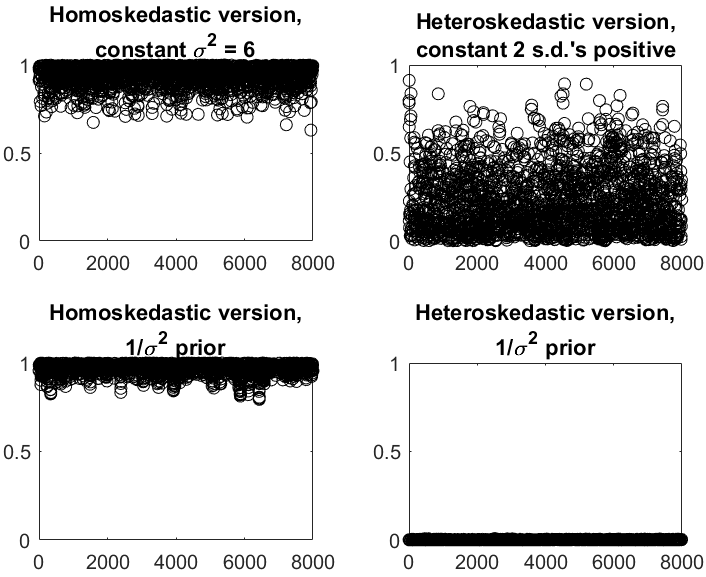
\includegraphics[width=.65\linewidth]{comp_obs_var}
\caption{MCMC results at various observation variance settings.}
\label{fig:comp_obs_var}
\end{figure}

\subsubsection{Full model and likelihood}
Blah

\subsubsection{Convergence difficulties}
% And the idea to eliminate boundary constraints
Blah

\subsubsection{Implementation of the Metropolis-Hastings algorithm}
Blah

\begin{figure}
\centering
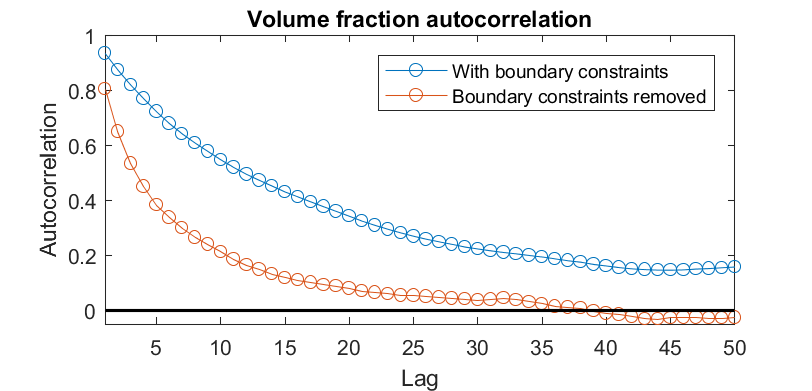
\includegraphics[width=.9\linewidth]{ACF_bnd_cnds_fig}
\caption{Auto-correlation for draws both with and without the elimination of boundary conditions.}
\end{figure}

\subsection{Which data to desire?}
Blah

\subsubsection{Motivations behind the choice of desired data}
Blah

\subsubsection{Differing results}
% for different desired data values
\begin{table}[h]
\centering
\begin{tabular}{| c | c  | c  |  c | c  | c | c | c |}
\hline
Desired data $d$ & $\sigma^2_{defl}$ & $\sigma^2_{rot}$ & $\sigma^2_{cost}$ & $\mu_{v|d}$ &
                            $\mu_{h|d}$ & $\sigma^2_{v|d}$ & $\sigma^2_{h|d}$\\
\hline
$(0, 0, 0)$ & 375.45 & 277.69 & 2.62 & 0.215 & $4.01 \cdot 10^{-2}$&
	$4.41\cdot 10^{-2}$ & $1.92 \cdot 10^{-3}$\\
$(0.65, 0.077, 96)$ & 16.74 & 15.25 & $4.62 \cdot 10^{-7}$ &
	$1.09 \cdot 10^{-3}$ & $3.36 \cdot10^{-4}$ &
	$1.02 \cdot 10^{-5}$ & $9.97 \cdot 10^{-6}$\\
\hline
\end{tabular}
\caption{Comparison of results for two different (low) values of $d$. Values listed are, respectively, the posterior means for the observation variance of each model output, posterior means for volume fraction ($v$) and thickness ($h$), and posterior variance of volume fraction and thickness.}
\label{table:d_comp}
\end{table}

\begin{figure}
\centering
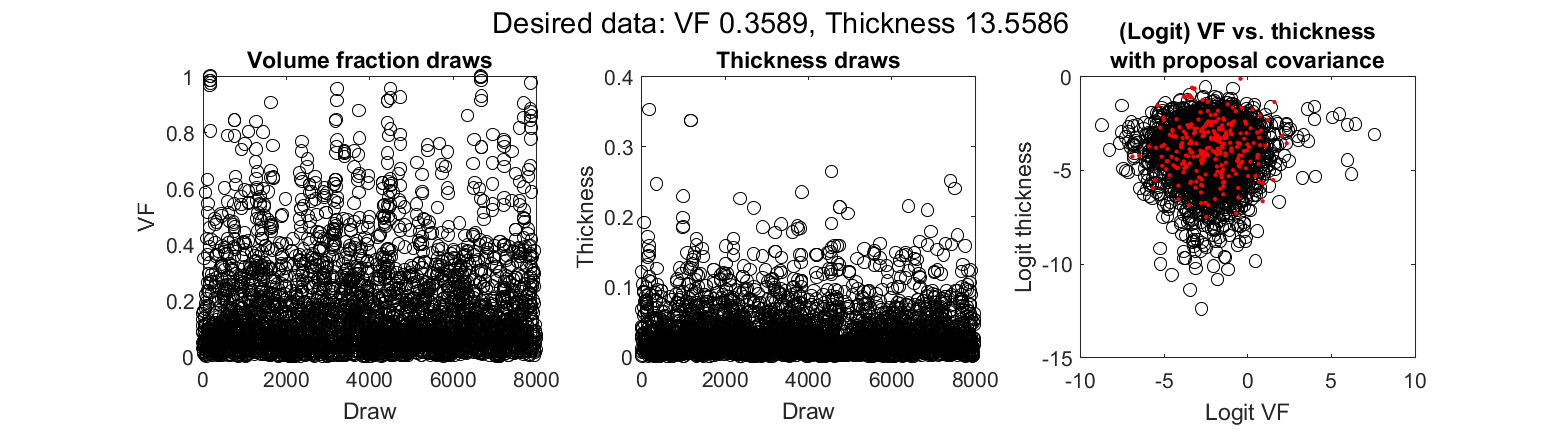
\includegraphics[width=.9\linewidth]{FIG1}
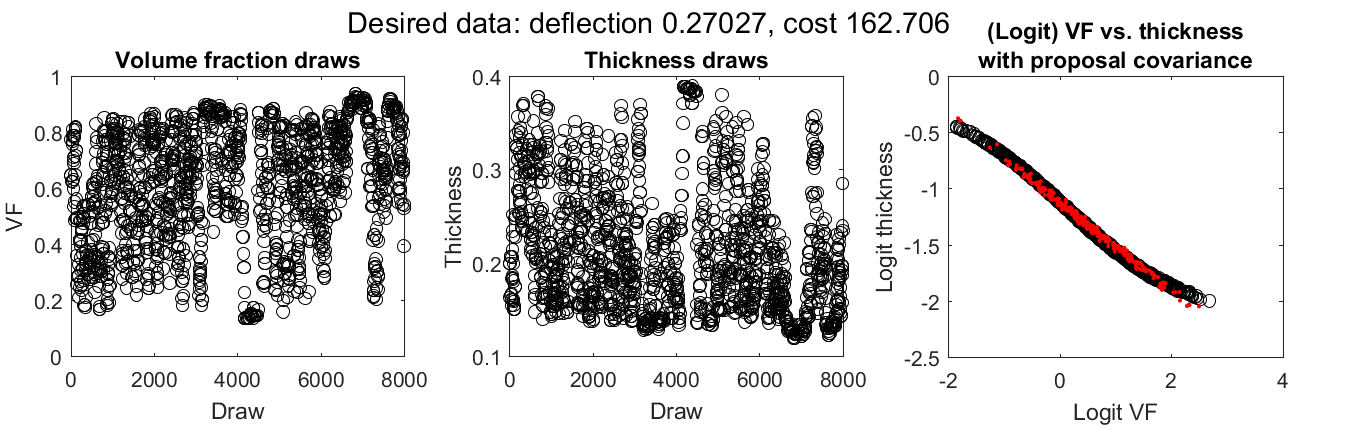
\includegraphics[width=.9\linewidth]{FIG2}
\caption{MCMC results for low deflection and cost (top row) and low deflection with easily achievable cost (bottom row).}
% NOTE: THESE PLOT TITLES ARE WRONG! GOTTA DO THE PLOTS OVER! LOL!
\label{fig:des_data}
\end{figure}

\subsection{Exponentially distributed desired data}
Blah

\subsubsection{Motivation}
Blah

\subsubsection{Implementation and results}
Blah


\subsection{Identifiability issues}
% Issues arising from the non-identifiability of VF, thickness when cost is relaxed
Blah

\section{Future work}
Blah

\subsection{Alternative means of handling cost}
Blah

\subsubsection{Removing cost from the model}
Blah

\subsubsection{Alternative priors for controlling cost}
Blah

\subsection{Building a desired data response surface}
Blah

\subsection{Implementing Hamiltonian Monte Carlo}
Blah

\subsubsection{Hamiltonian Monte Carlo}
% Background
Blah

\subsubsection{Benefits}
Blah

\subsection{Model discrepancy}
% Include (or investigate the inclusion of) a model discrepancy function
Blah

\section{Conclusion}
% Discussion of the role of computer model validation as a potential methodology for design
Blah












\bibliographystyle{plain}
% This style file is a version of the plain.bst style file which I edited myself to add abstract and annotation fields.

%\bibliography{lit_review}

\end{document}